%Introductory sentences here

Below, we list the key elements of data collection in simulation. In Section \ref{subsection:environment}, we talk about the features of our virtual setup. Section \ref{subsection:dataCollection} includes information about the methodology driving data acquisition, as well as the data structures. 

\subsection{Features and Constraints of the Virtual Environment}
\label{subsection:environment}

\begin{itemize}
\item MuJoCo \cite{MuJoCo} has been chosen as the base physics simulator. 
\item 3D Models 294 objects of 20 classes have been retrieved from online repositories.
\item Each 3D model is decomposed into convex parts using V-HACD method \cite{V-HACD}.
\item Distributions of weight and dimensions for each object class has been determined using real-world data. These distributions are later used in simulation to sample realistic objects.
\item MuJoCo is configured to use an impedance controller to control the DLR-II hand in simulation.
\item In order to simulate the Carmine 1.09 depth sensor installed on the robot, a modified version of \cite{KinectSimulator} has been used. 
\item The variations used in each scene consist of camera position, orientation and distance from the object, as well as object weight, friction, scale, location and orientation. 
\item A near-perfect 3D model of DLR-II hand has been used to simulate the robotic hand. There are no kinematic constraints on how the hand can grasp an object, other than collisions with the virtual table where the objects reside. 
\end{itemize}

In order to create a realistic simulation environment, we chose MuJoCo \cite{MuJoCo} physics simulator over other simulators/game engines OpenSim, BulletPhysics, ODE or NVIDIA PhysX, due to two reasons: 
\begin{itemize}
\item MuJoCo uses generalized coordinates and optimization-based contact dynamics, resulting in less numerical instabilities,
\item MuJoCo is optimized for quality of physics as well as speed, hence improving the quality of the physics simulation.
\end{itemize}

Due to the fact that MuJoCo needs objects to consist of convex parts for collision checks, all 294 objects in the 3D model dataset has been approximately decomposed into convex parts. Fig. \ref{fig:objectDecomposition} approximate decompositions of some objects in our dataset, using V-HACD algorithm \cite{V-HACD}. The number of sub-parts for all objects in our dataset varies between 2-120, depending on the complexity of each object. 

\begin{figure}
  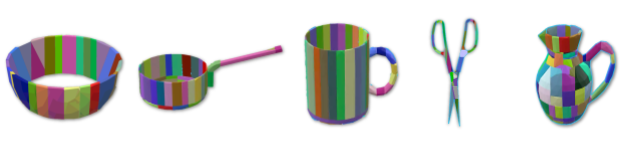
\includegraphics[width=\linewidth]{images/decomposition.png}
  \caption{Approximate convex decomposition of some objects in our dataset. Best viewed in colour.}
  \label{fig:objectDecomposition}
\end{figure}

The dataset of objects include bottles, bowls, cans, boxes, kitchen utensils, mugs, cups, pans and other graspable objects such as tennis balls and dust pans, as seen in Figure \ref{fig:allObjects}. All objects used in the simulation are chosen to be within the grasp affordance limits of the DLR-II hand. Our shape collection dataset consists of 294 objects from 20 classes. The number of objects in each class varies between 25 (bottles) and 1 (dustpan). 250 objects from all classes have been used for training the network, while the remaining 44 has been used for validation in simulation. The objects included in simulation are graspable everyday objects having different characteristics. Examples are kitchen objects such as bowls, plates, mugs and teacups, solid objects such as boxes and balls, kitchen utensils such as spatulas, spoons. Long/thin objects such as spatula, fork, spoon, knife classes are placed on a heavy cup vertically in order to make them graspable without touching the table. 

\subsection{Data Collection Methodology}
\label{subsection:dataCollection}

In order to fully learn the relationship between visual cues, grasp parameters We have chosen not to consider the kinematic constraints of an attached robotic arm. We considered the hand as having a free joint where the only constraint on its movement is collisions with the table where the objects stand on. We divided the data collection process into units called \textit{scenes}, where each scene has a single object placed on a table, and a number of grasps are attempted to pick up the object. Below, we specify the time flow of data collection:

\begin{enumerate}
\item A novel instance of an object from the dataset is generated and placed on a virtual table. Variations applied include object position, orientation, scale, weight and friction coefficients.
\item A simulated depth camera takes a depth image $I_s$ of the scene, converting it into a point cloud $P_s$. The ${elevation}_s$ of the camera view point varies between 30-57 degrees, whereas the ${azimuth}_s$ is sampled from $[0, 2\pi]$. 
\item The grasp generator algorithm by Kopicki et al. \cite{kopicki2015ijrr} is used to generate a number of candidate grasps $H = \{h_i\}_{i=0}^{K}$. Top 10 grasps from all 10 categories is picked and applied to the object in simulation.
\item More simulated depth images are taken from other virtual cameras around the object. The location and orientations of these cameras are determined based on the same distribution where the initial image was taken, as explained in step 2. Up to 20 images are acquired, and a random view is associated with each grasp created in step 3. 
\item Results, including grasp success outcome, grasp information and depth image are stored for every trial. The grasp parameters are converted to the frame of reference of the associated view for every grasp.
\end{enumerate}

Each candidate grasp $h_i = \{w_0, ..., w_{n}$ consists of a series of 10 waypoints along : $w_0$, ..., $w_{n}$. A waypoint $w_k$ is a 27-element vector that specifies full configuration of the hand in joint space: 3 dimensions for 3D coordinates and 4 dimensions for the orientation of the wrist, and 20 parameters specifying each finger joint's activation. 

After a grasp $h_i$ is generated in world coordinates, the waypoints that belong to the grasp are converted to the camera's frame of reference. The key goal of our network architecture is to learn which grasps are more likely to succeed given a point cloud, where both input channels are represented in terms of the camera frame of reference. This point differentiates us from the work of Levine et al. \cite{Levine1}, where camera coordinates are not used. It should be noted that the possible camera locations in our simulated data covers a larger space, with full circular movement $[0, 2\pi]$ on azimuth and $[30-57]$ range in elevation. Our scenes do not have any distinguishing landmarks such as a bin or robot base, which may aid the network in locating the camera in the scene. 

In each scene $S_i$, a number of depth images are taken $\{I_{ik}\}_{k=0}^20$, in the manner explained above. The first image $I_{i0}$ is used to generate grasps, as explained in Section \ref{section:generative}. We use up to 20 distinct views in each scene, while we typically perform 100 grasps. Attaching different views to each grasp instead of using the seed image $I_{i0}$ ensures there is more variation in terms of viewpoints, resulting in a richer dataset. 20 has been chosen as a compromise between 1 and 100, as sampling a view per grasp would introduce a large overhead. Typically, performing a grasp takes half of the time it takes to acquire an image using the simulated camera.

Once a grasp is performed in simulation, it is considered a success if an object is lifted 1 meters above the table, and held there for 2 seconds. If the object slips from the hand during lifting or holding operations and falls, the grasp is considered as failure. If the hand is still holding the object at the end of the duration, the grasp is considered as success. 

Describe the method for creating the simulation so that it matches the real world. Database of objects. Estimating ranges for object mass, friction, pose variation. Simulation of depth camera images. Assumptions about mass distribution, hand modelling and modelling of articulation and dynamics. Creation of simulated grasp data set.

\begin{figure}[t]
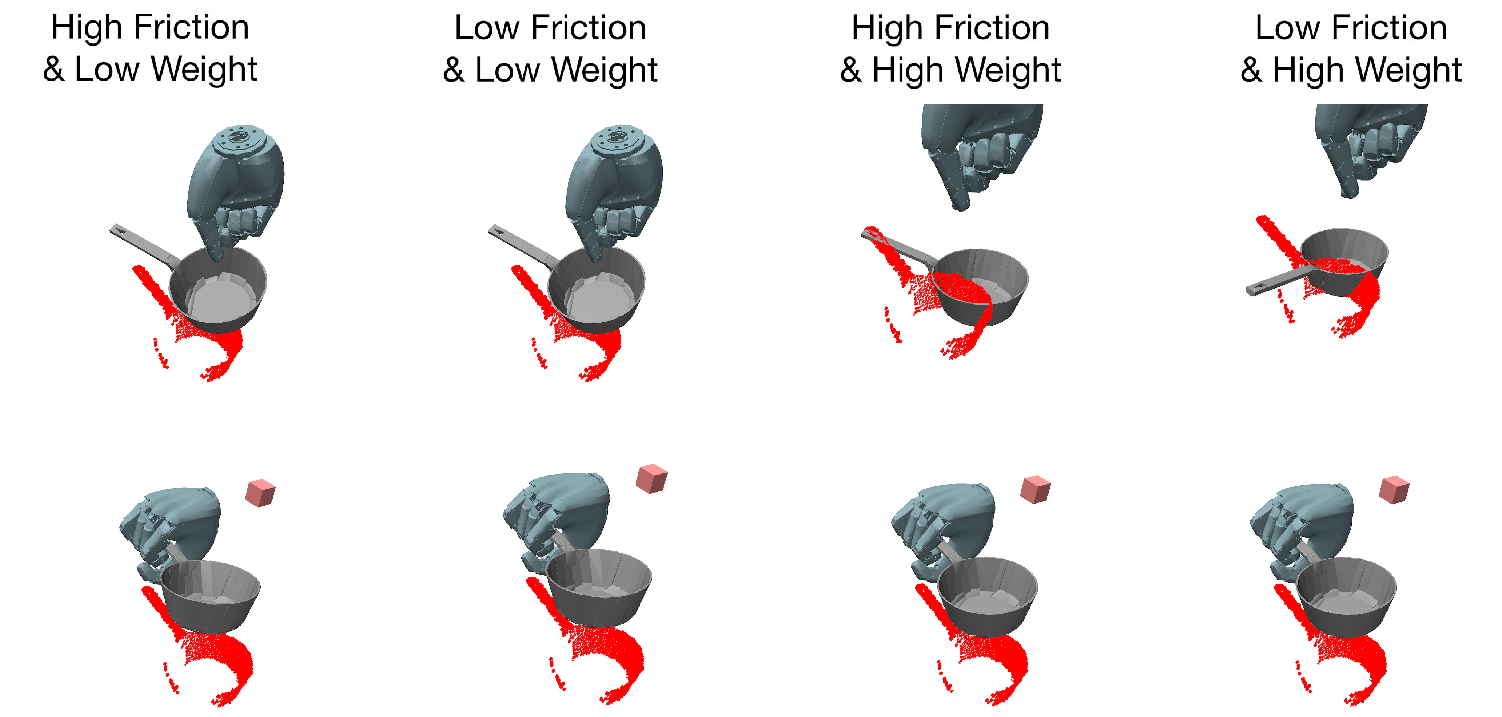
\includegraphics[width=\columnwidth]{images/frictionweight}
%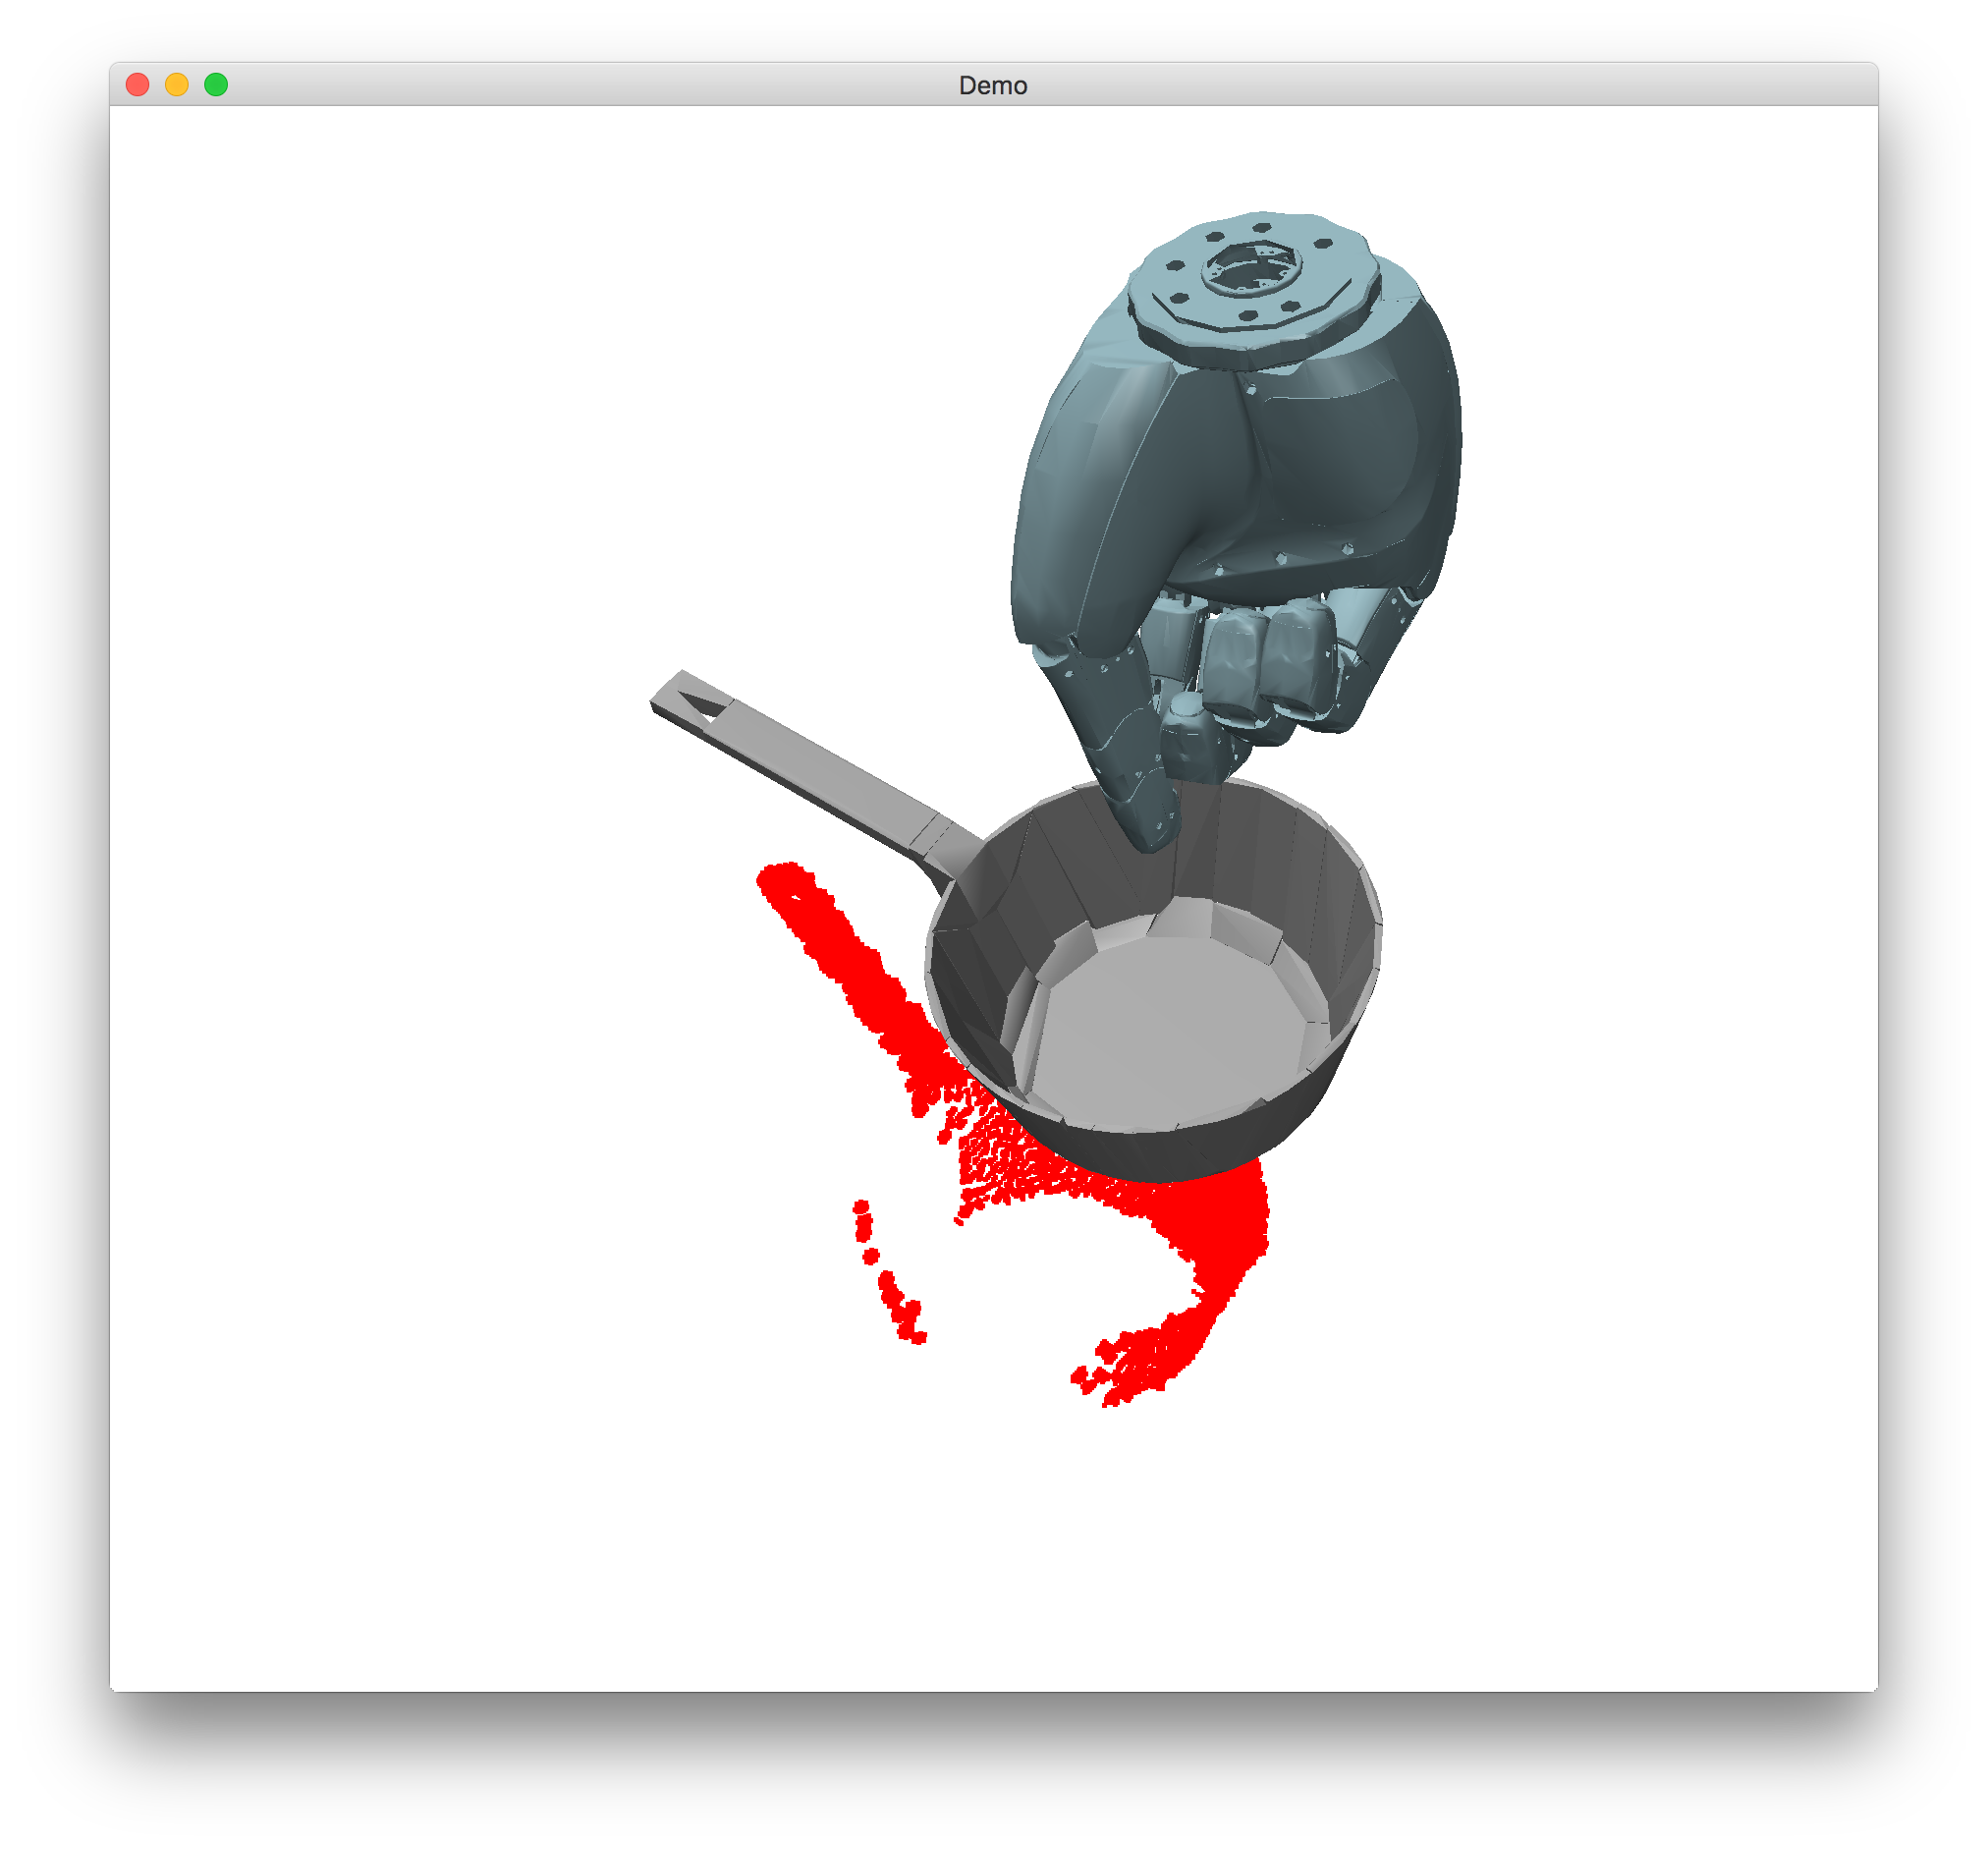
\includegraphics[width=0.24\textwidth]{images/Pan4_2_HFLW}
%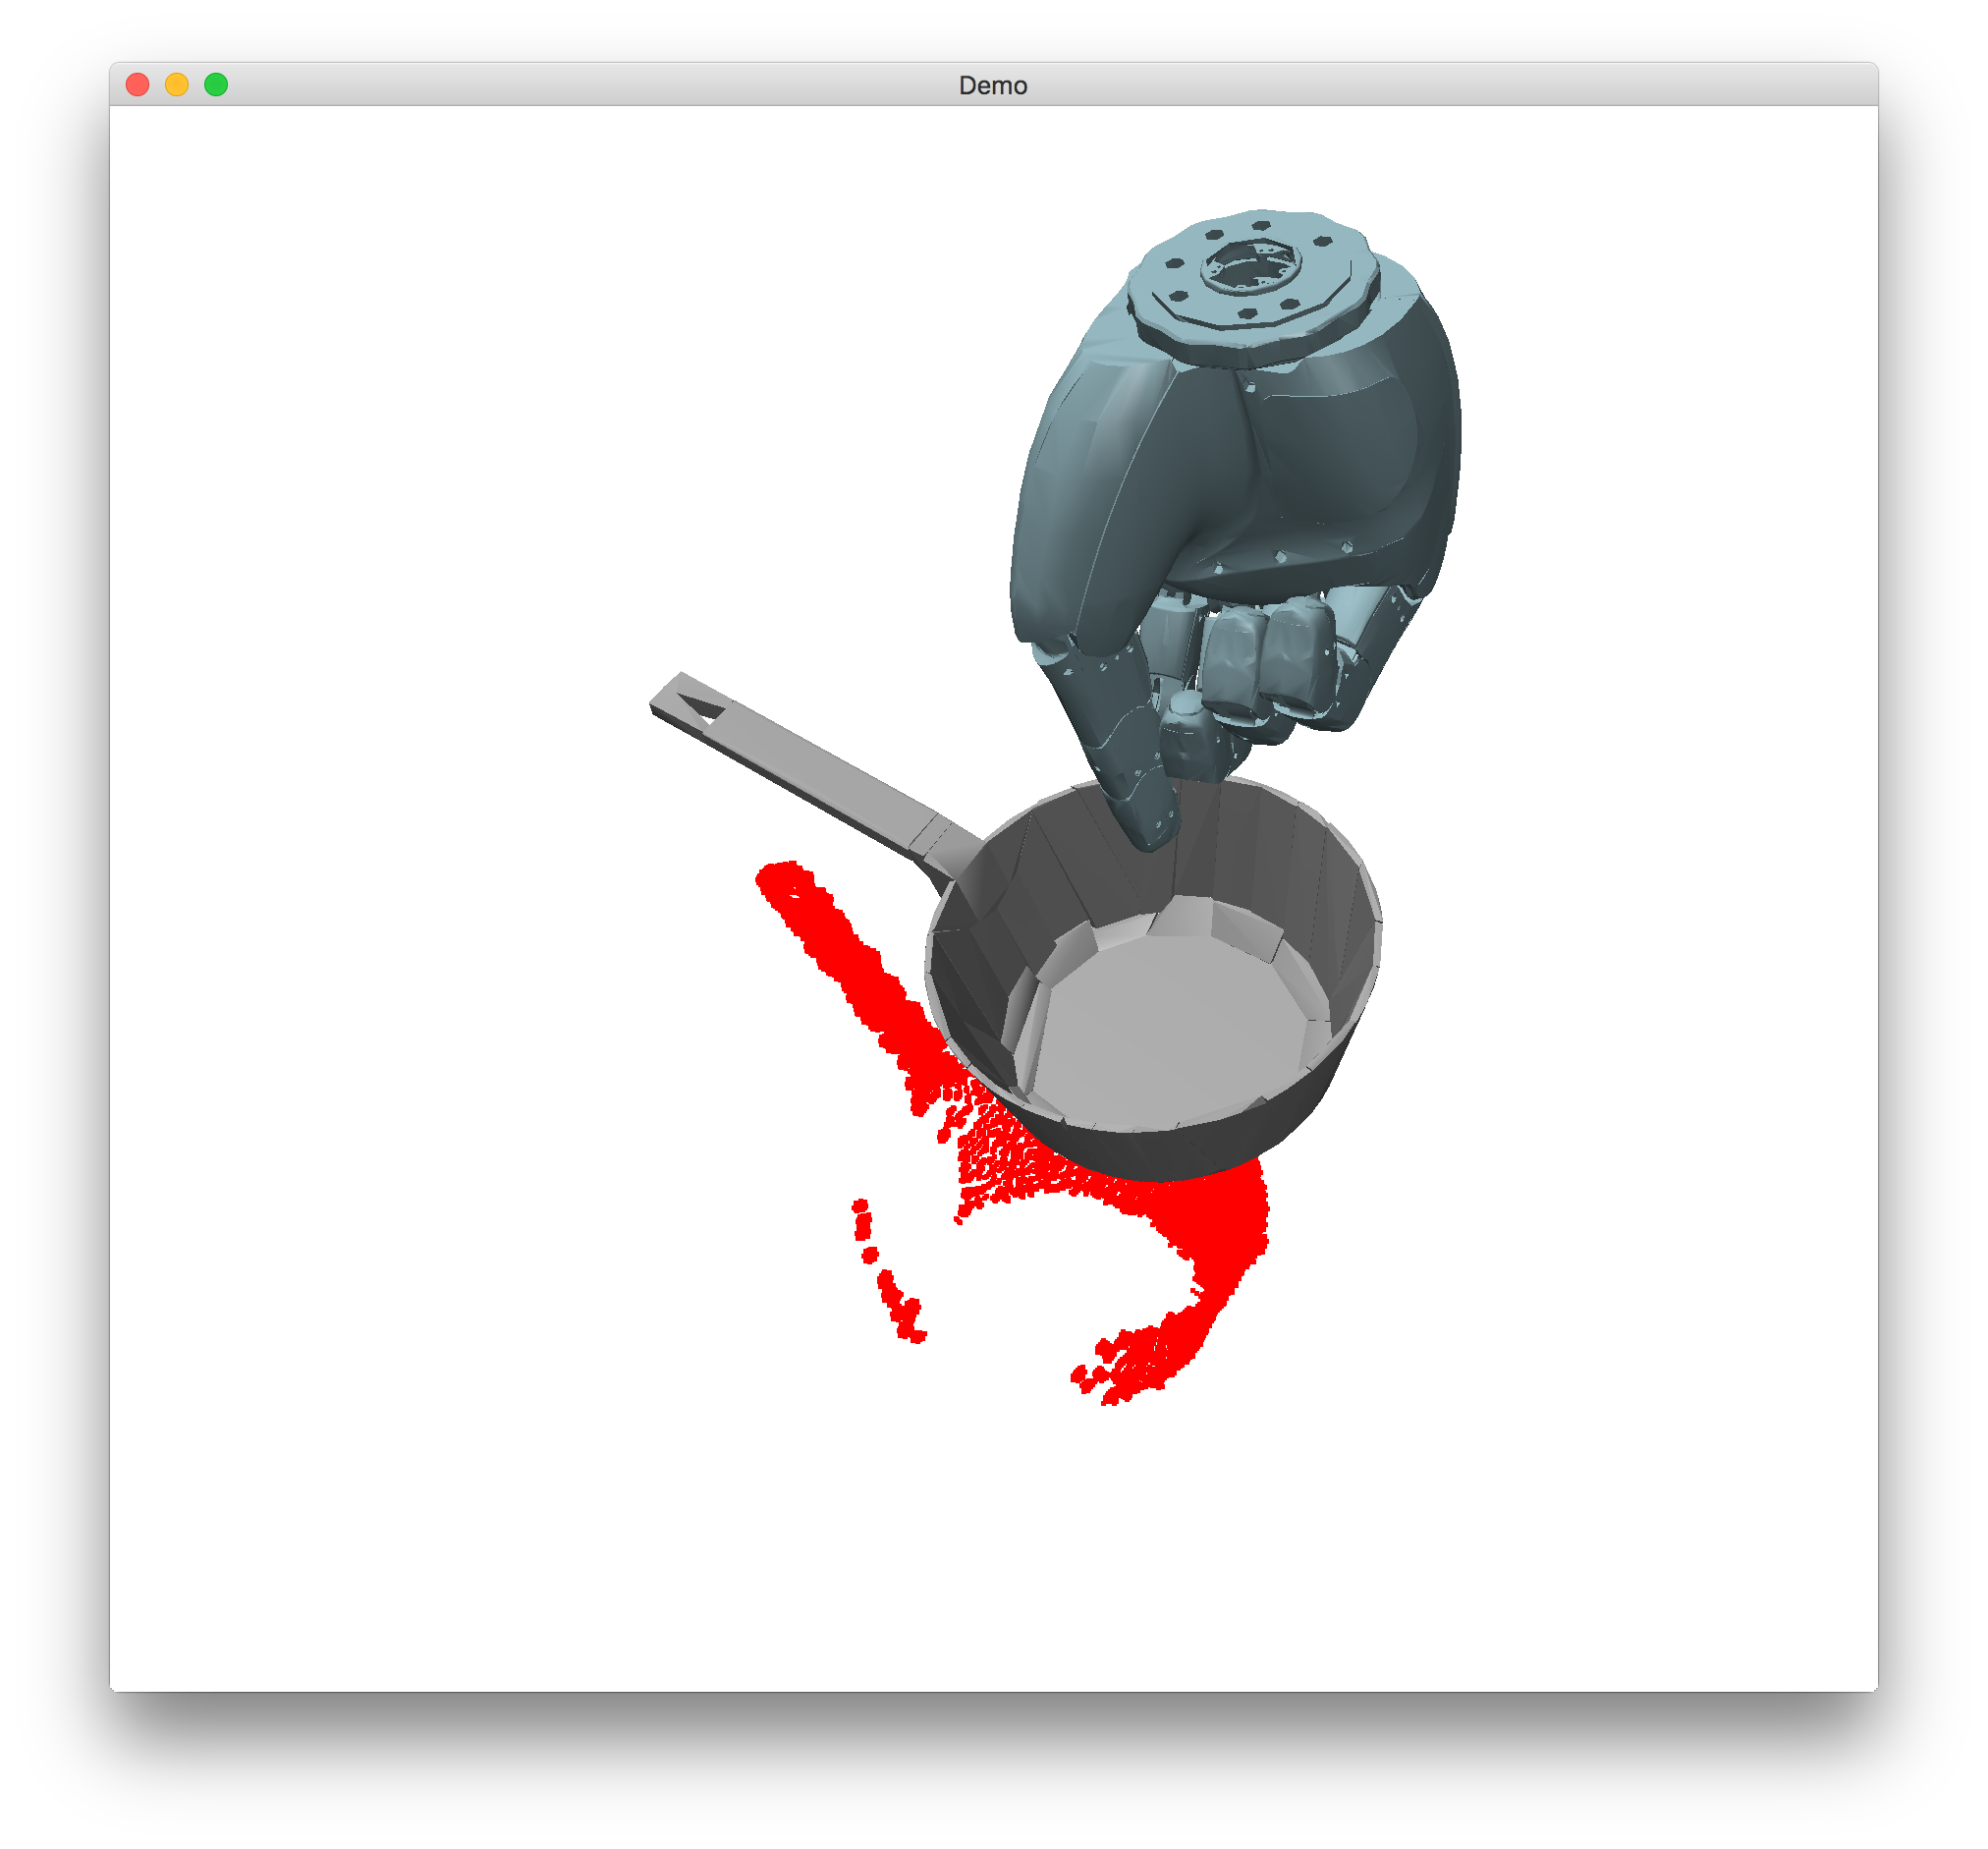
\includegraphics[width=0.24\textwidth]{images/Pan4_2_LFLW}
%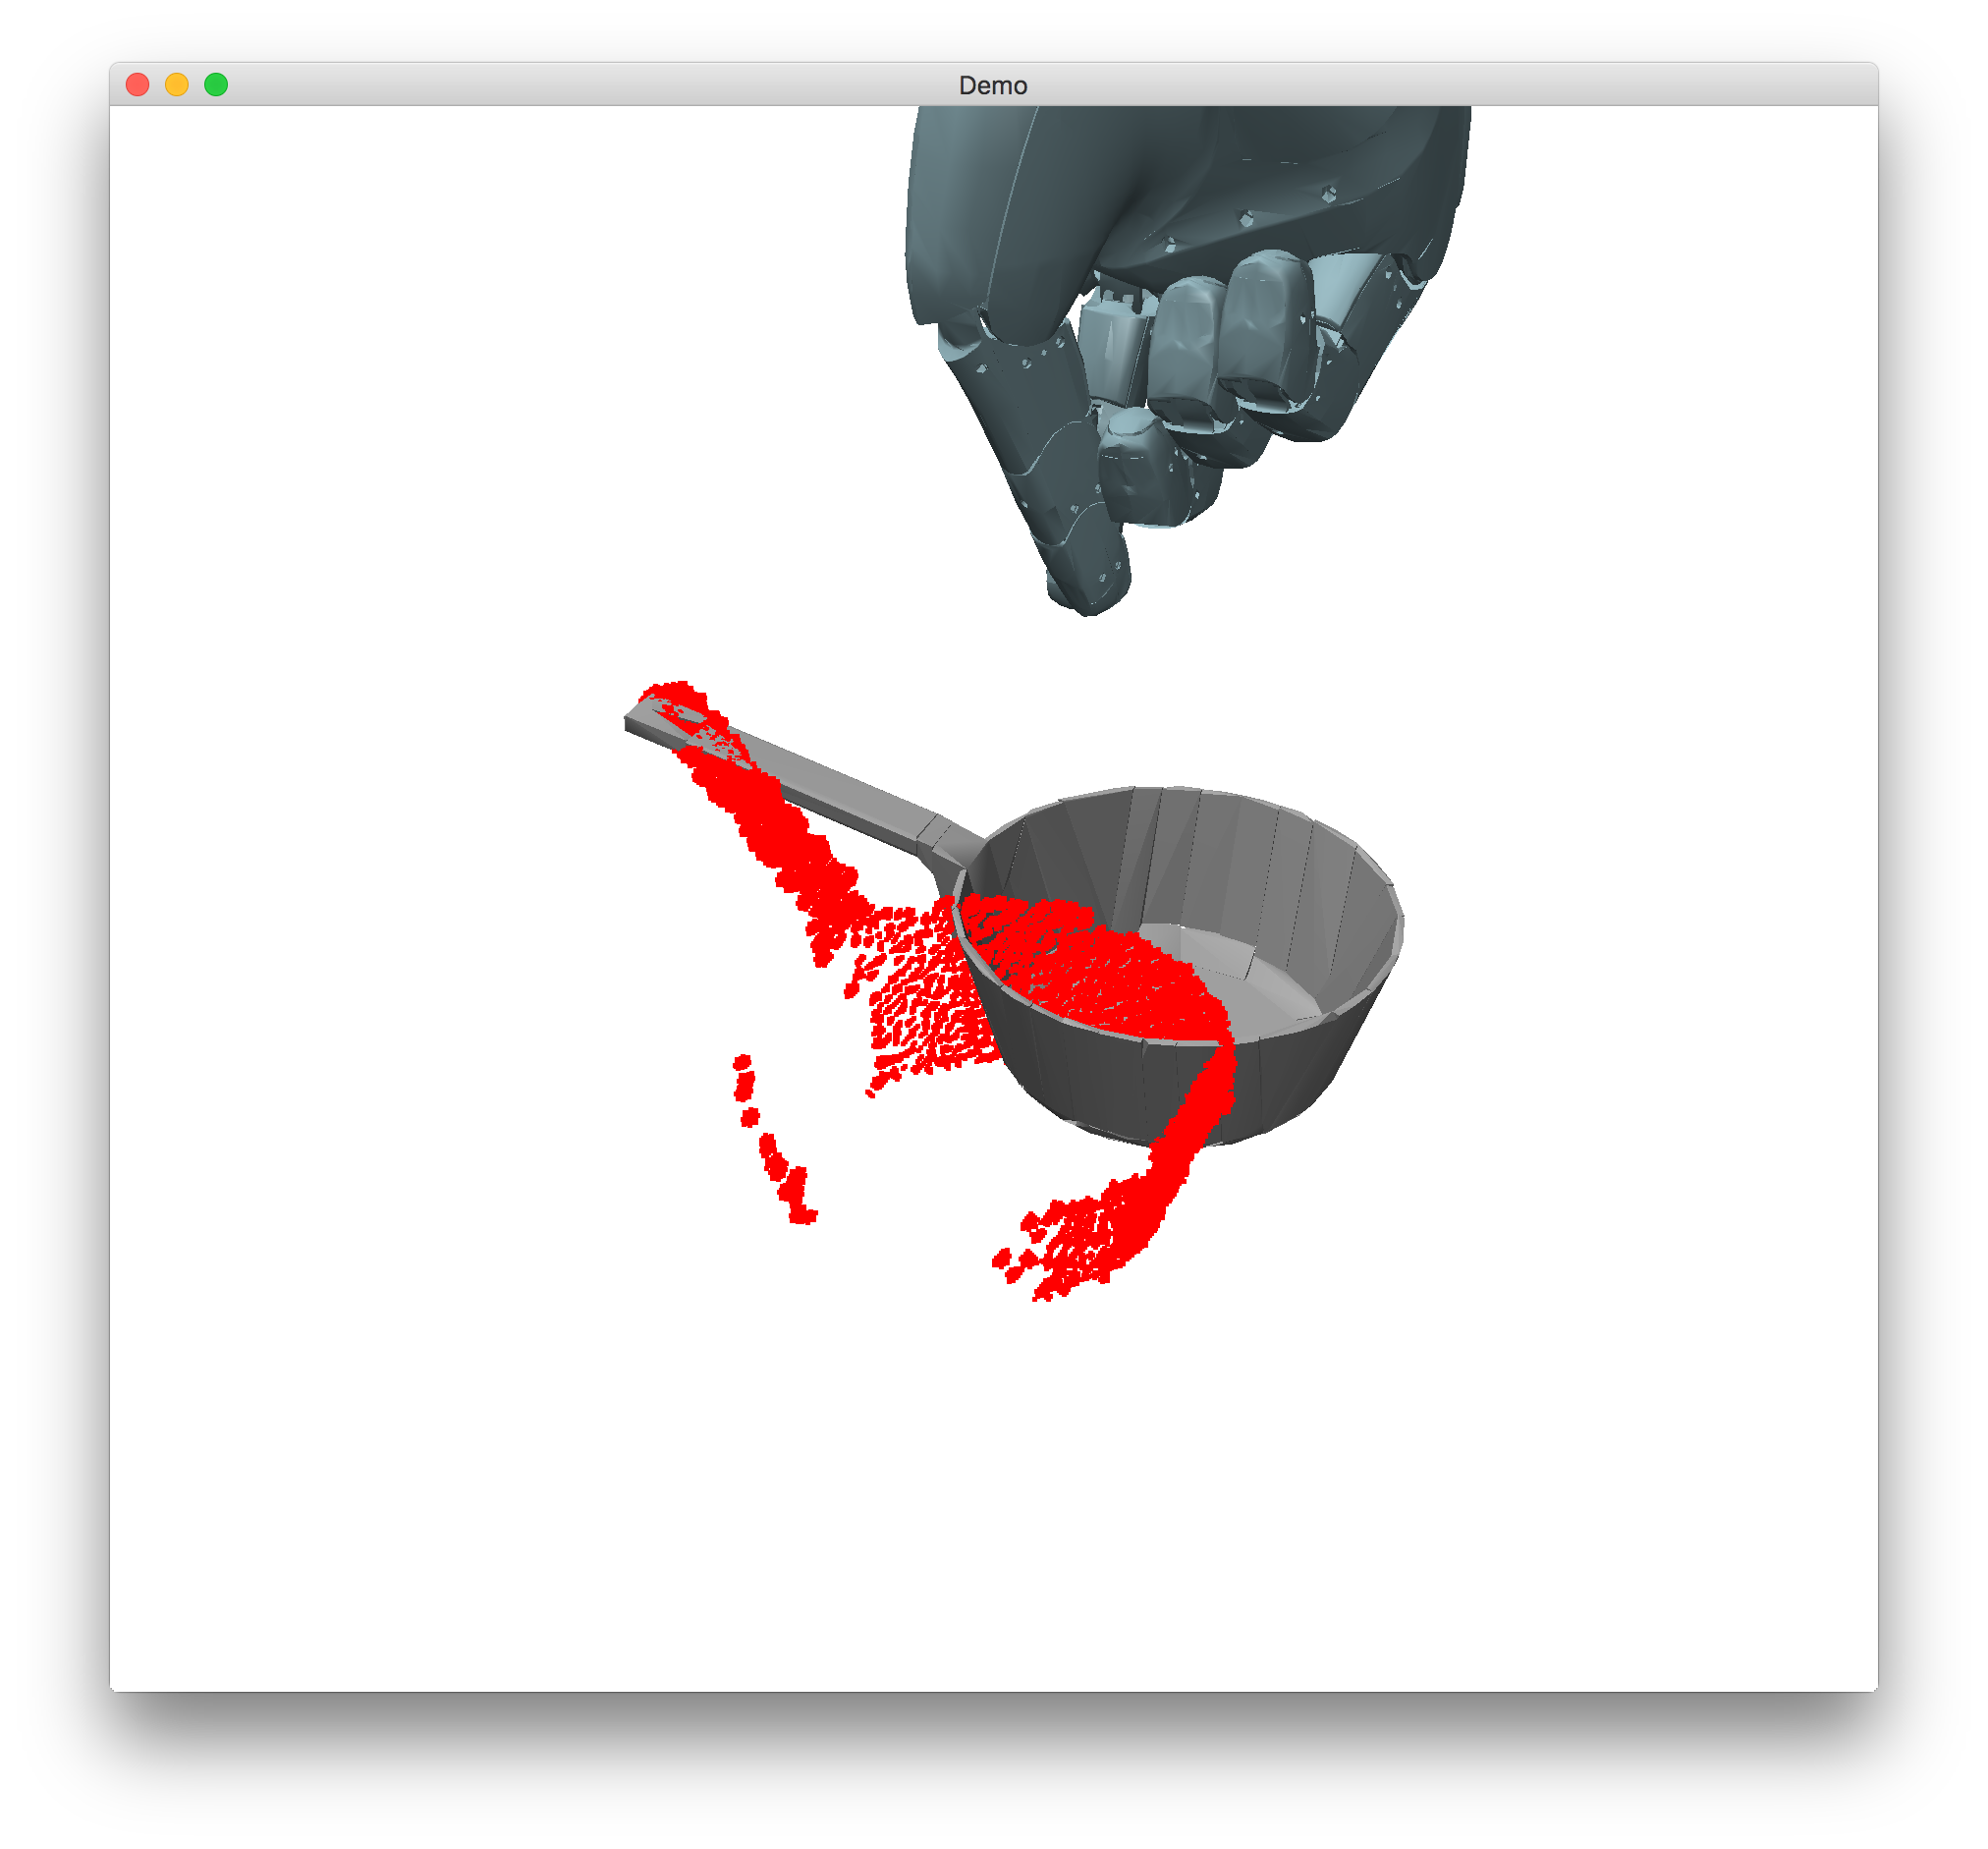
\includegraphics[width=0.24\textwidth]{images/Pan4_2_HFHW}
%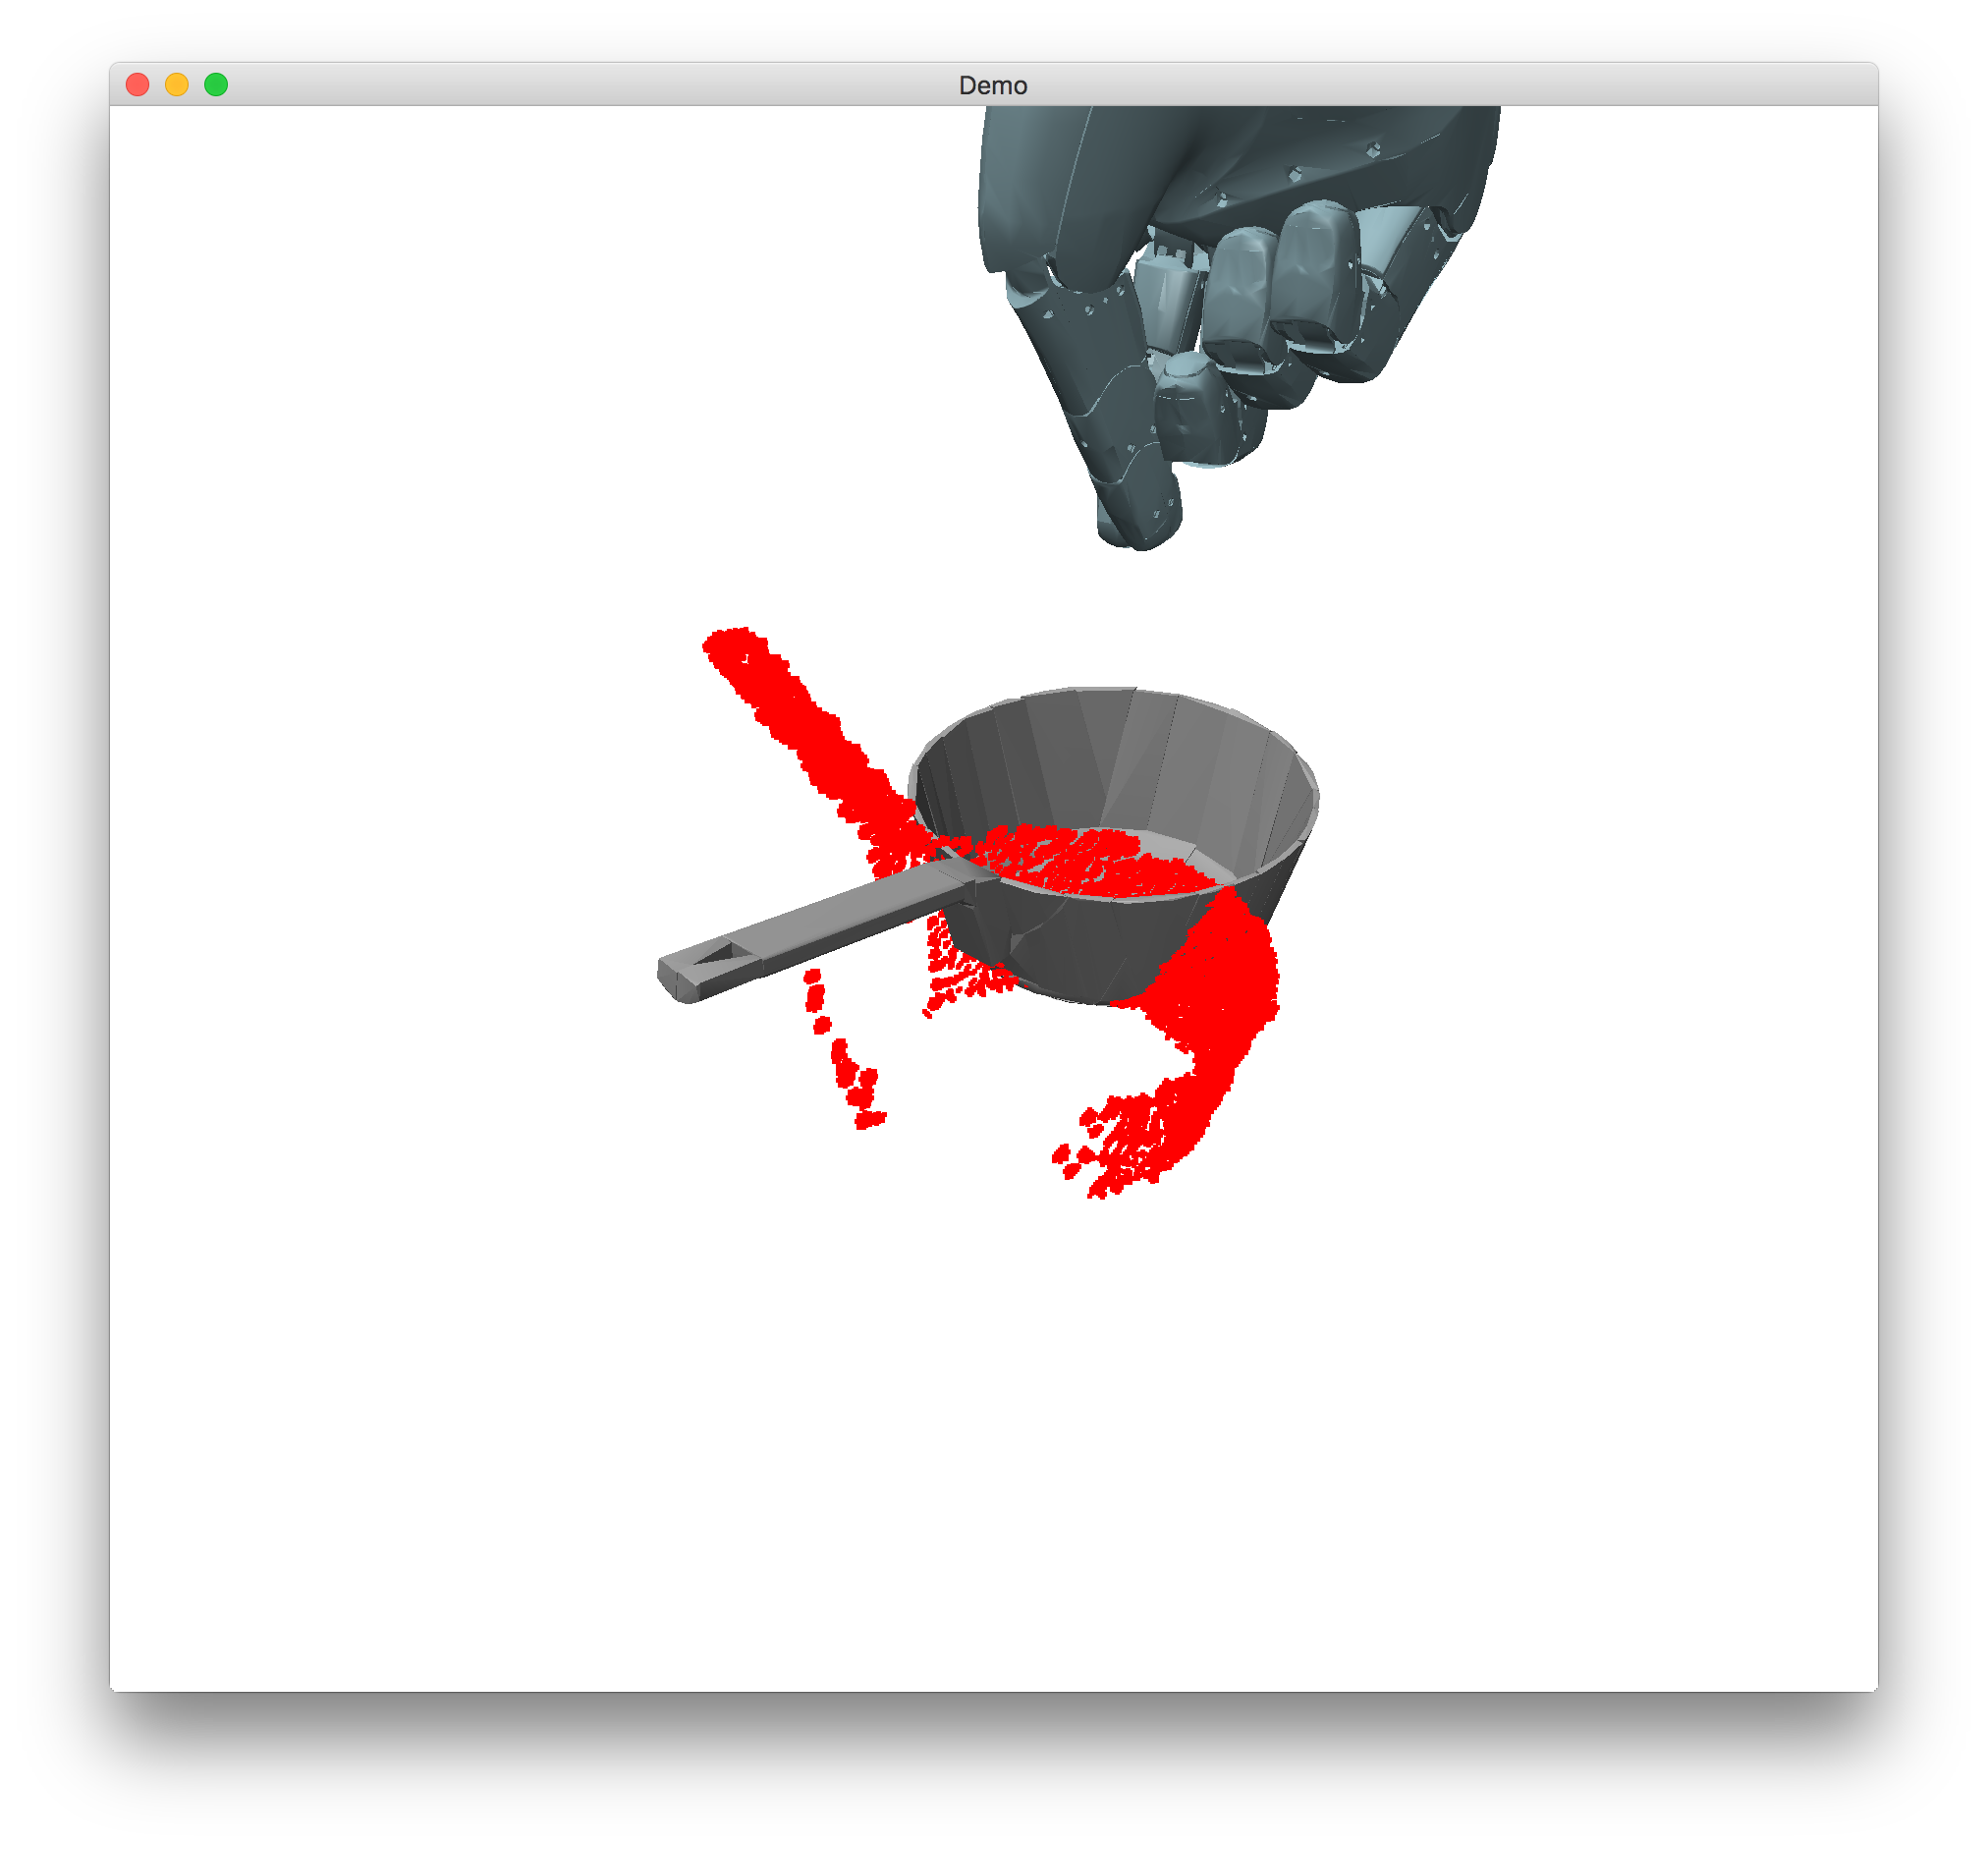
\includegraphics[width=0.24\textwidth]{images/Pan4_2_LFHW}\\
%%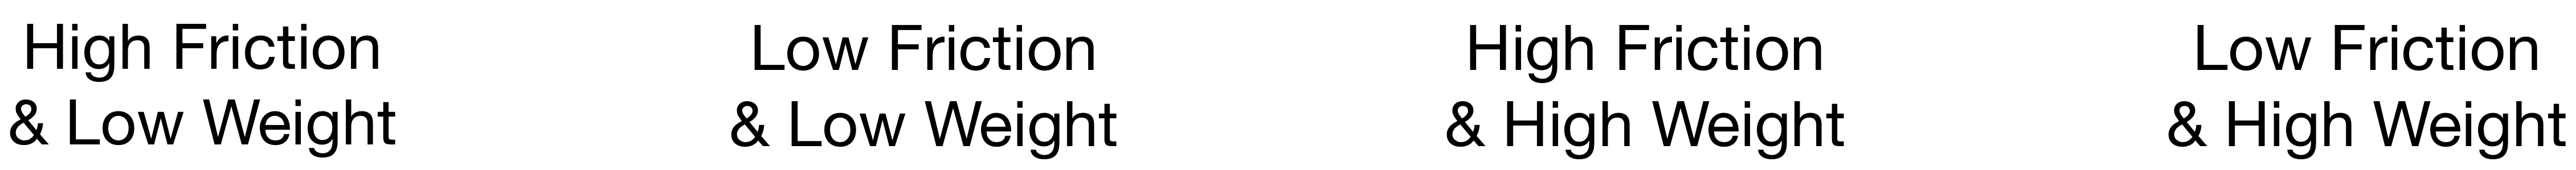
\includegraphics[width=0.96\textwidth]{images/key-to-eval-training}\\
%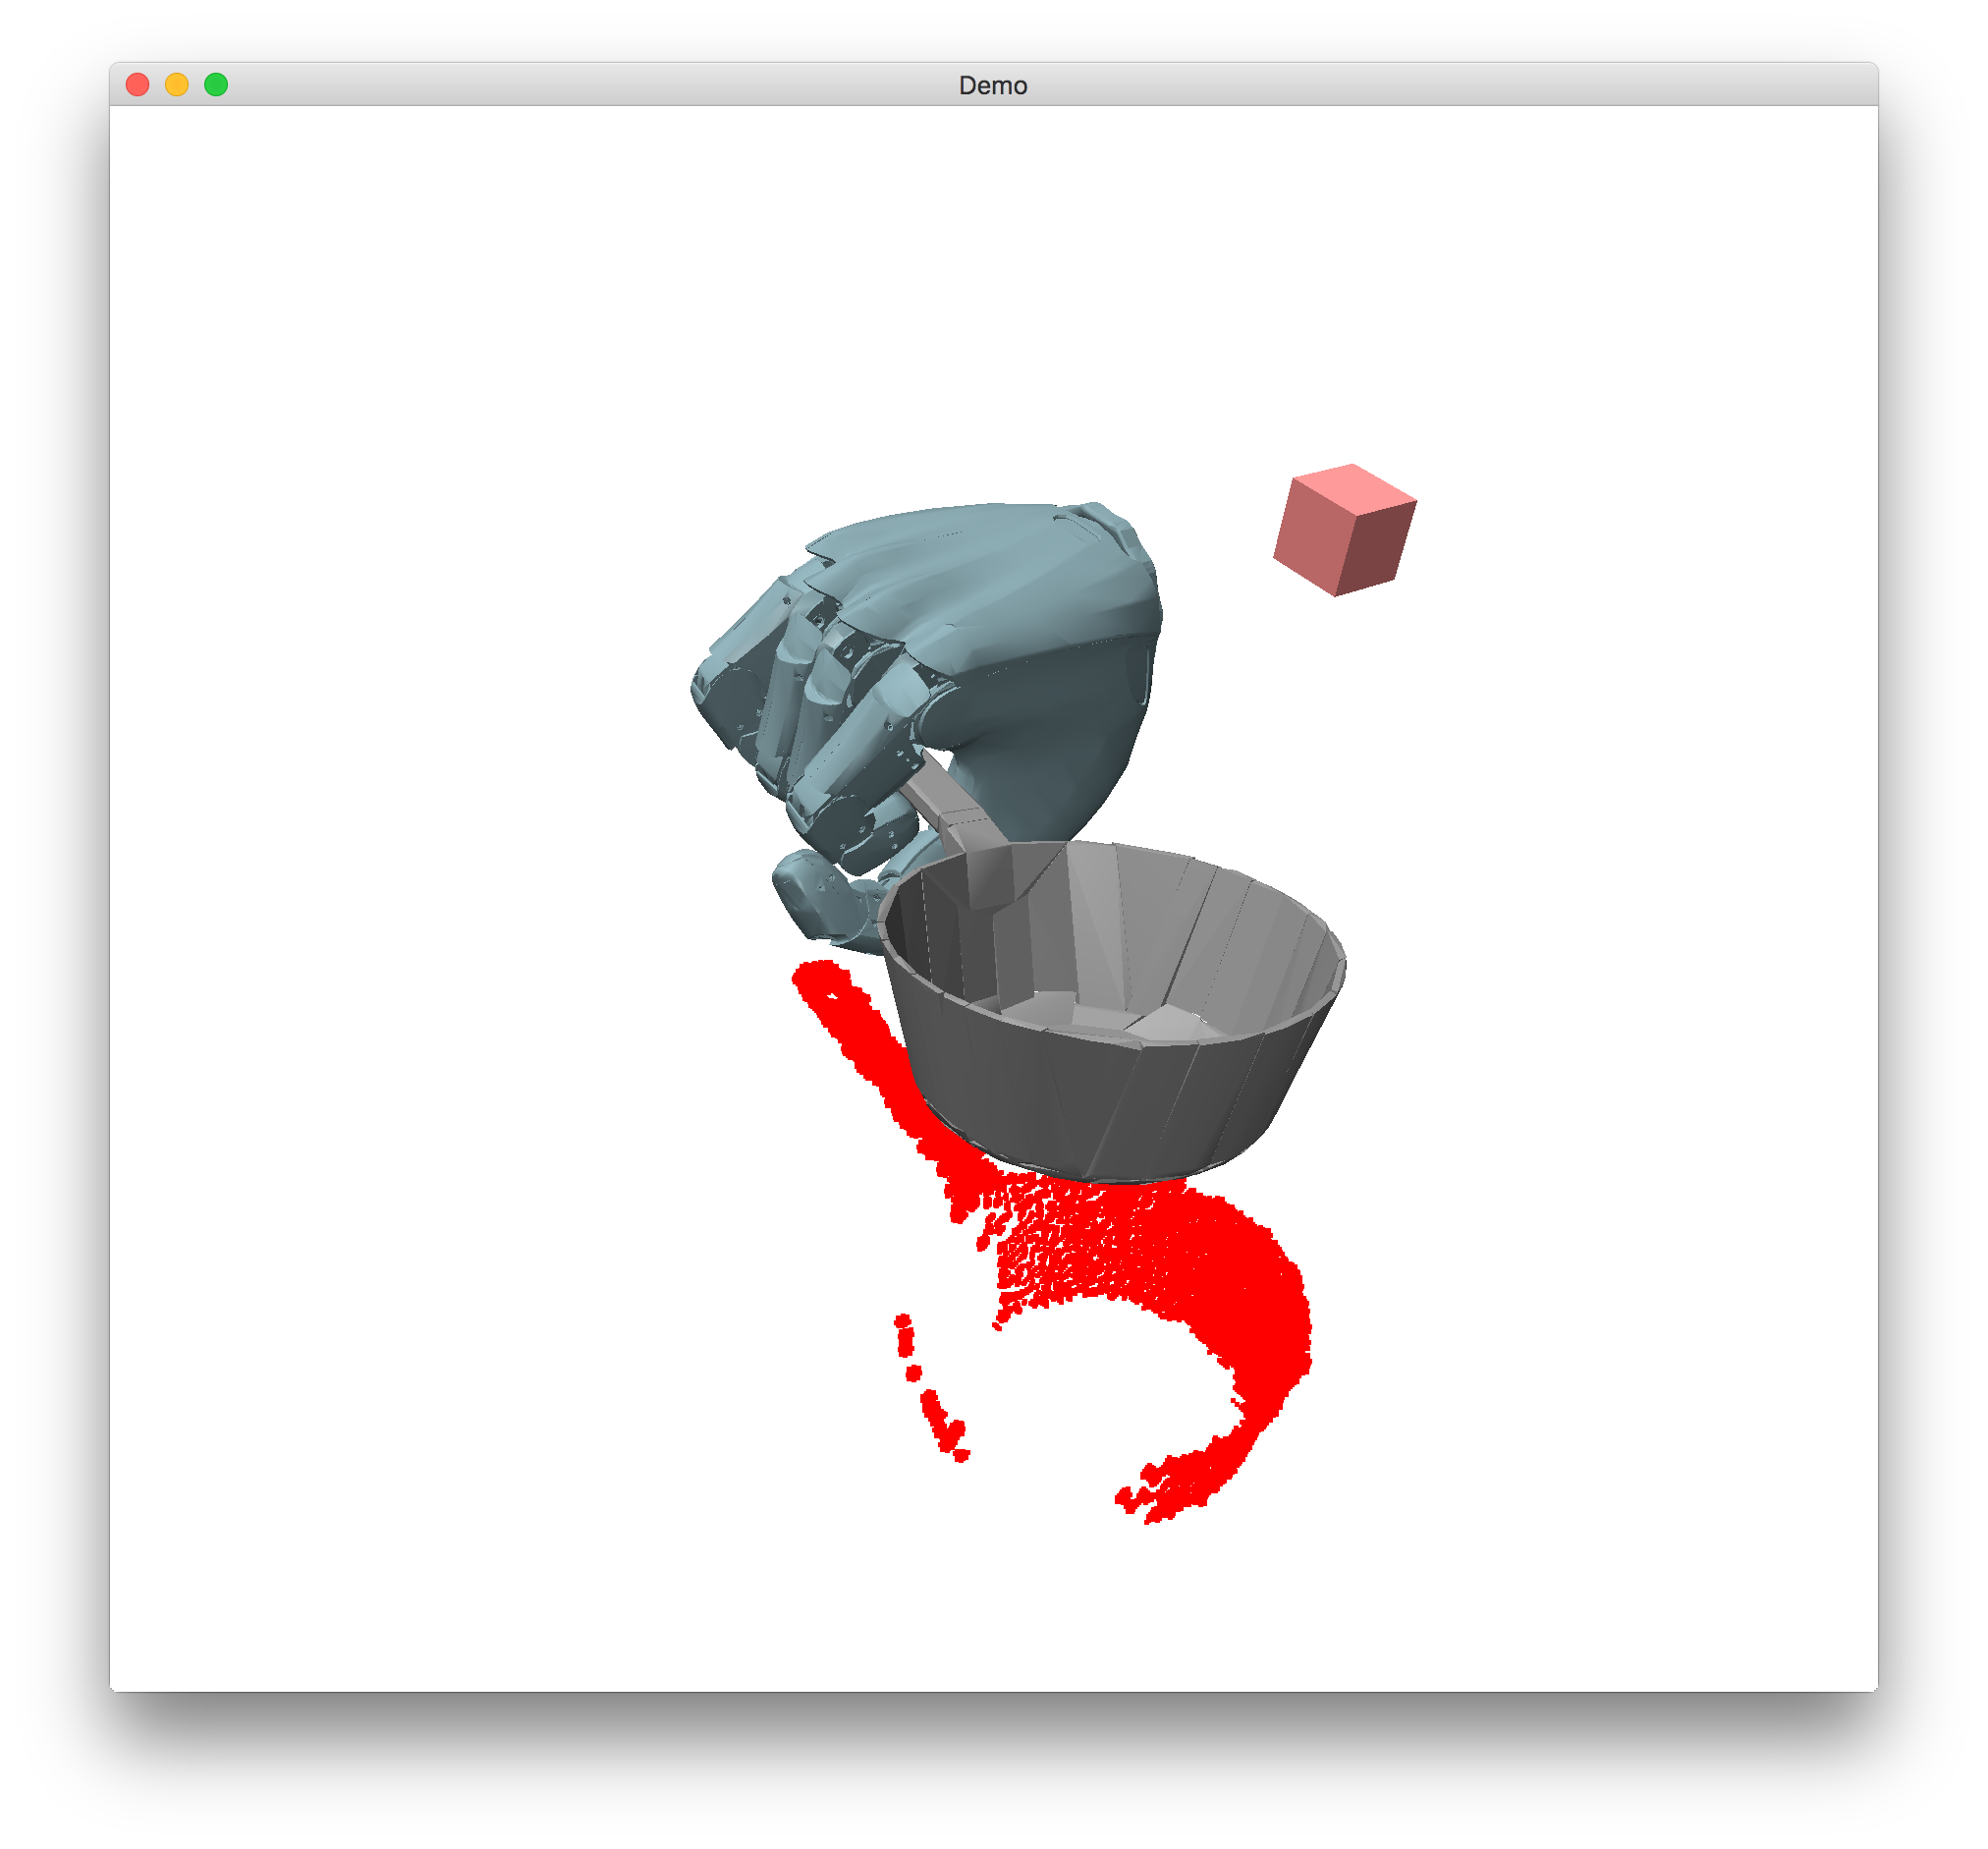
\includegraphics[width=0.24\textwidth]{images/Pan4_HFLW}
%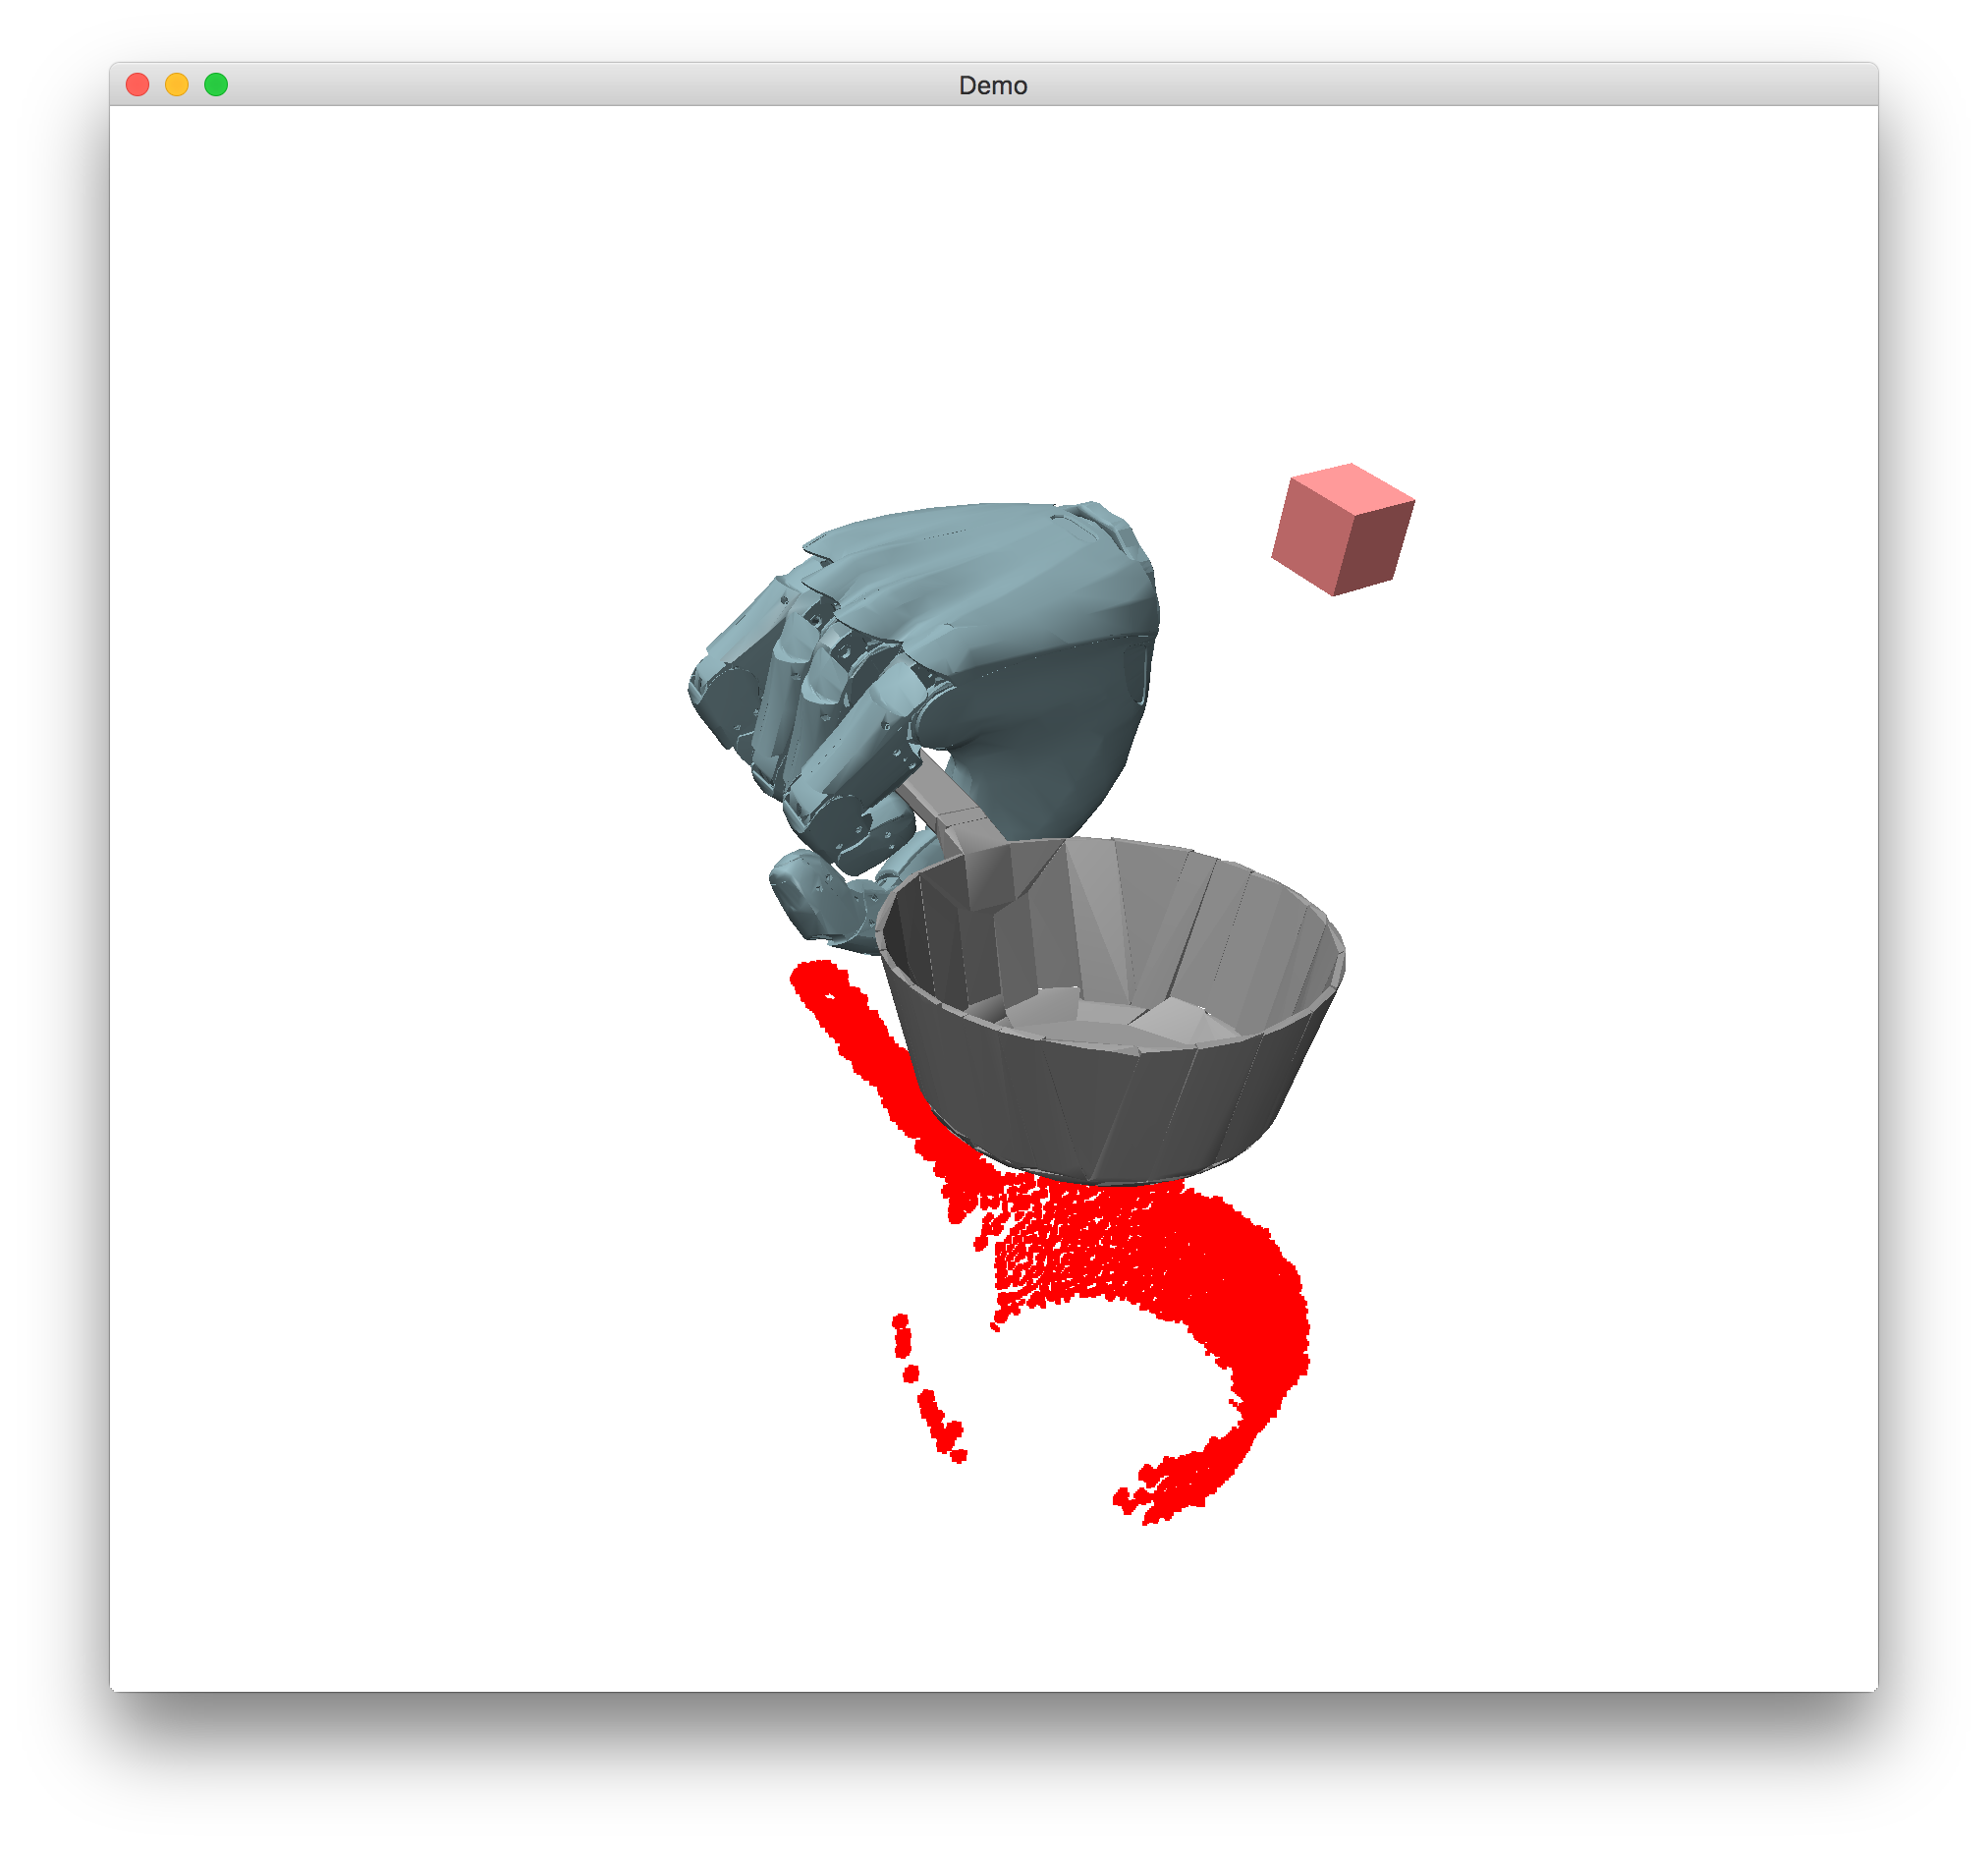
\includegraphics[width=0.24\textwidth]{images/Pan4_LFLW}
%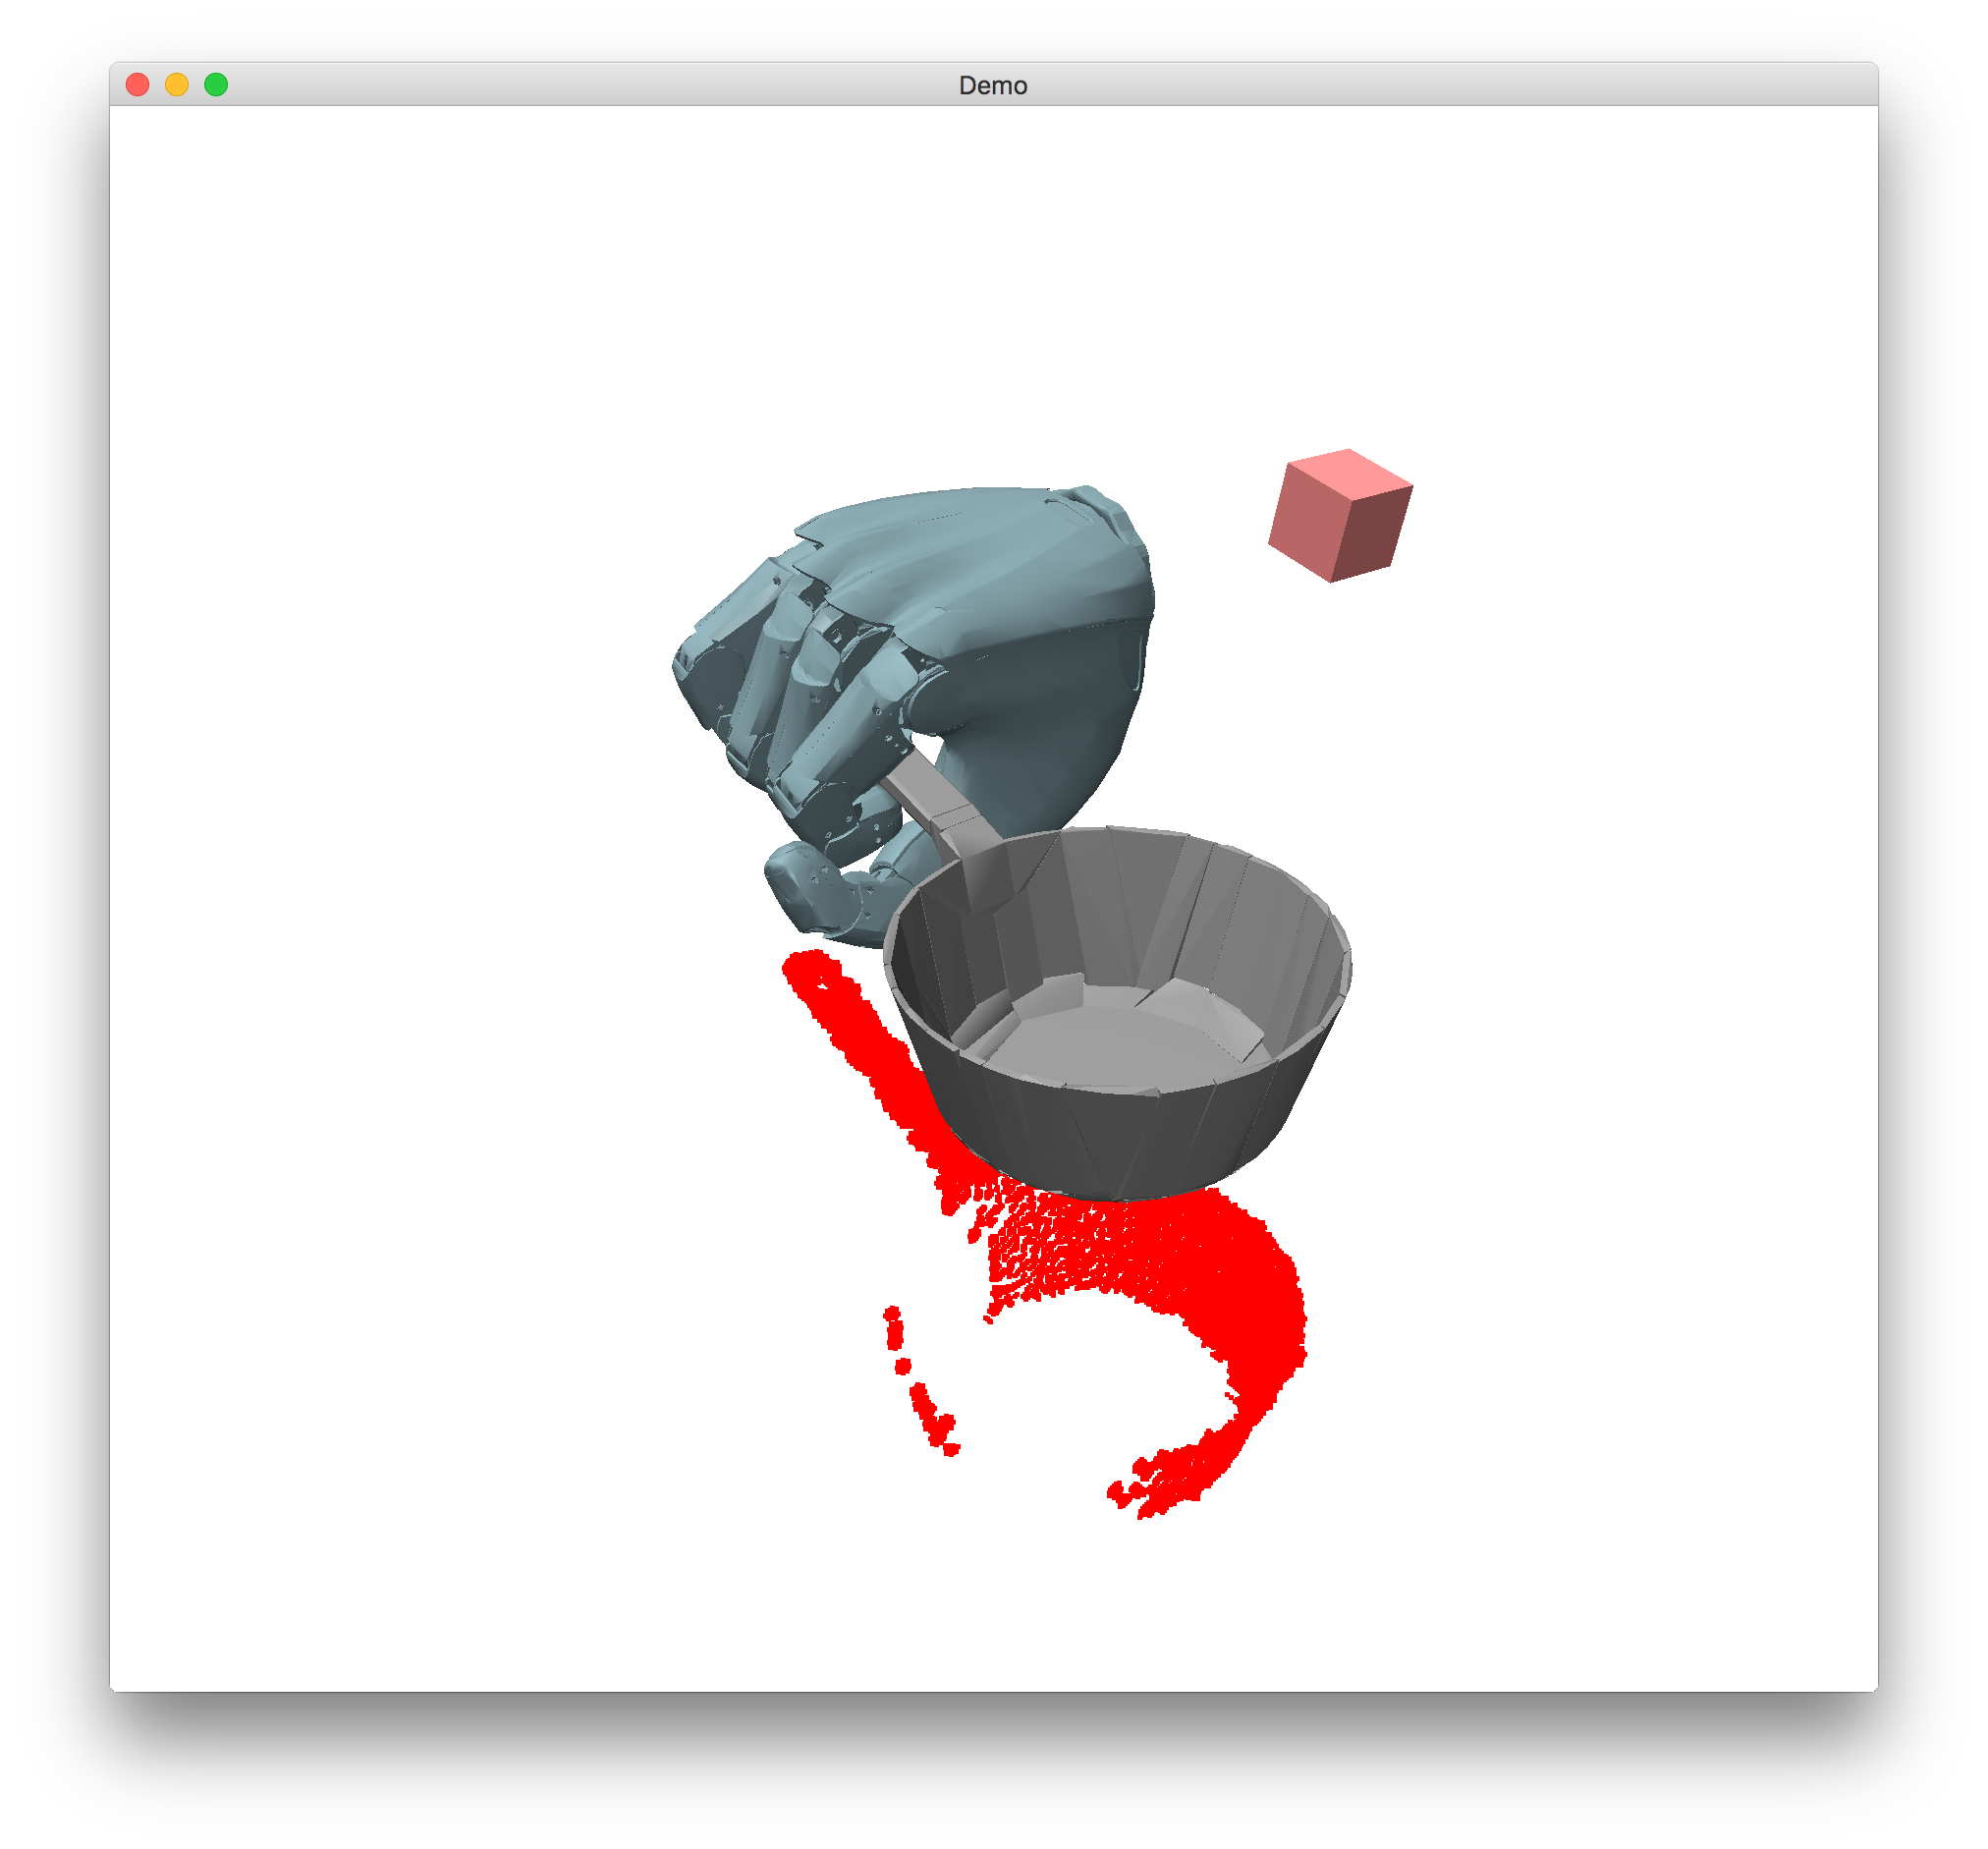
\includegraphics[width=0.24\textwidth]{images/Pan4_HFHW}
%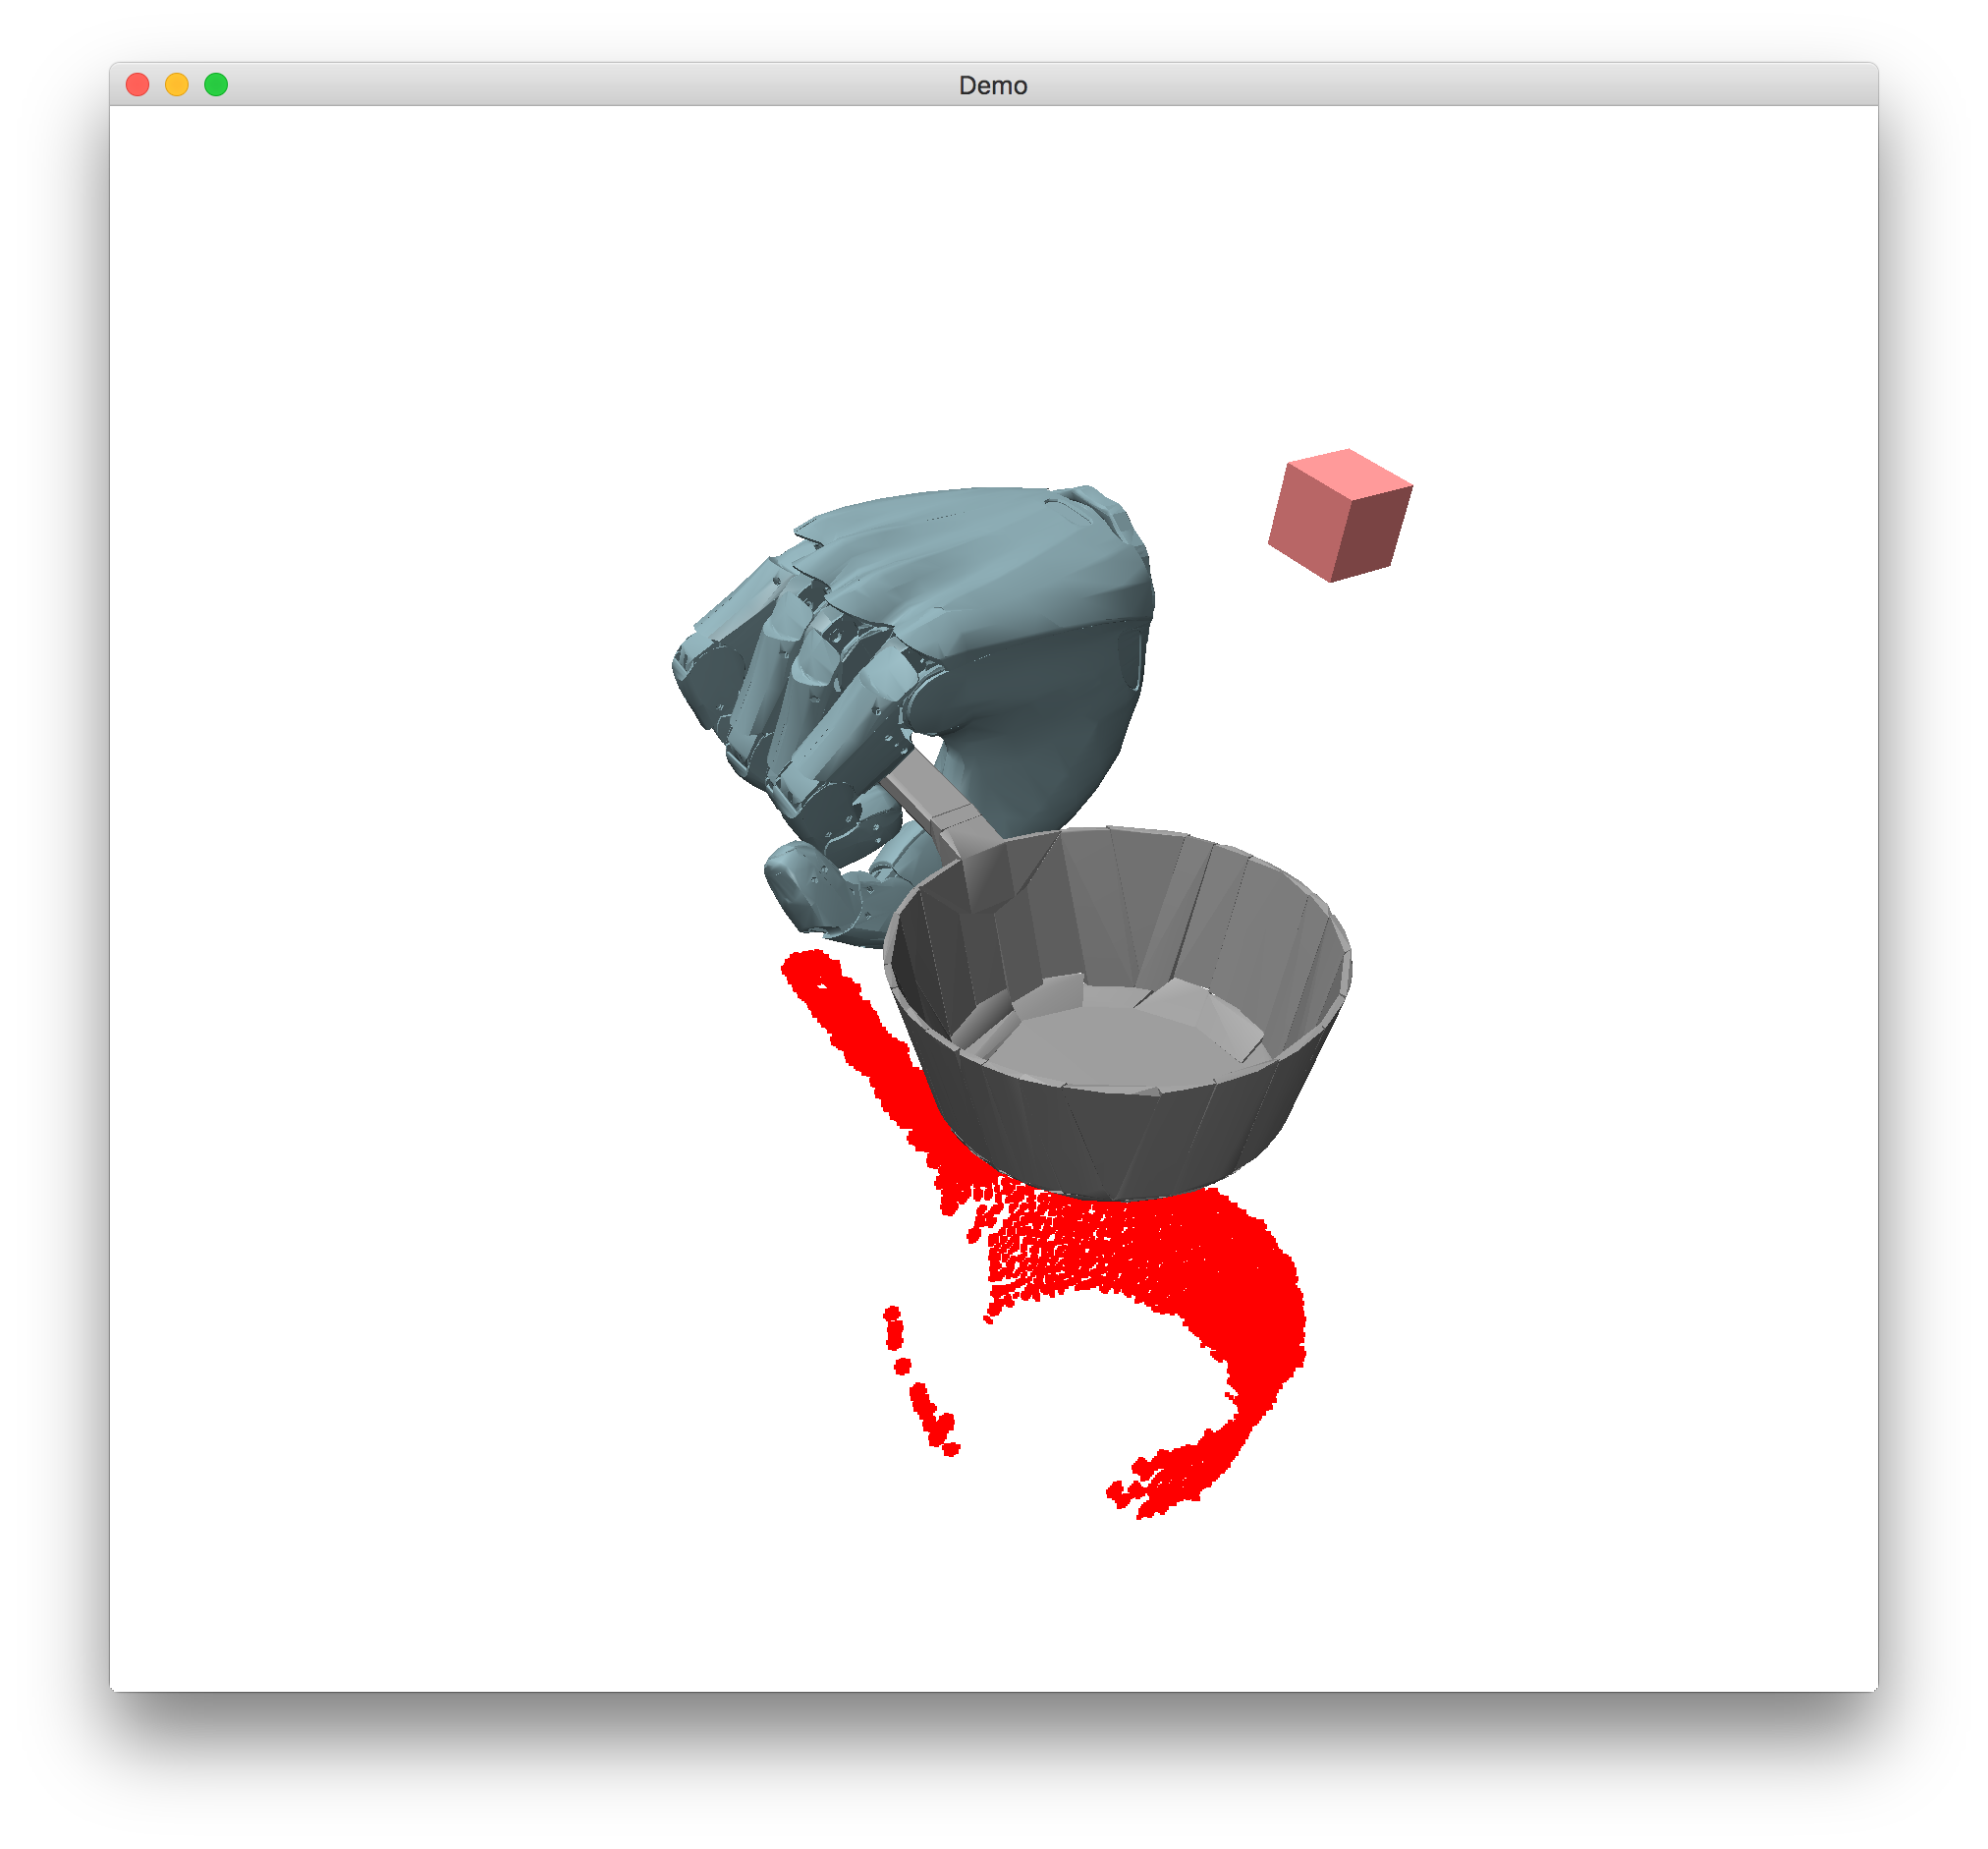
\includegraphics[width=0.24\textwidth]{images/Pan4_LFHW}
\caption{Training a robust evaluation model. (Top row) The same pinch grasp, executed on the same object, with varying friction and mass parameters. (Bottom row) A more robust power grasp, executed on the same object, with the same variation in friction and mass. \label{fig:evaluative-training}}
\end{figure}
